\newpage
\section{Plan dalszego rozwoju}
Możliwość łatwego rozwijania aplikacji była wielokrotnie wspominana w rozdziale \ref{sec:opis} jako cel projektowy uzasadniający wybór zastosowanych rozwiązań. W następującej części modyfikacje będą ułożone w kolejności od najprostszych do trudniejszych w realizacji.

Zakłada się że użytkownik aplikacji prowadząc własne badania, będzie mógł łatwo zastosować własne funkcje oceniające w trakcie działania aplikacji. Gdyby modyfikacja serwera oceny nie była preferowaną formą implementacji, wszystkie dane dostępne na bieżąco są także zapisywane do plików zapisu lotu w celu późniejszej obróbki. Podobnie, korzystając z edytora poziomów aplikacji Unreal Engine, oraz obiektów przygotowanych przez autora, można w graficzny sposób ułożyć różne nowe zadania zawierające przeszkody, trajektorie lotu i inne obiekty wizualne.

Kolejnym elementem łatwym w modyfikacji jest model dynamiczny statku powietrznego. Dzięki separacji od reszty systemu, możliwy jest wybór dowolnej symulacji obsługiwanej przez środowisko ArduPilot. Wśród alternatywnych programów do symulacji można wymienić m.~in. X-Plane-10, Gazebo, oraz MATLAB Simulink. Oprócz narzędzi dostępnych od twórców oprogramowania ArduPilot, dowolne oprogramowanie wykorzystujące protokół MAVLink może być podłączone. \begin{todo}Stosując odpowiedni program tłumaczący możliwe jest podłączenie także komercyjnego oprogramowania FLIGHTLAB praca Łukasza\end{todo}.

\begin{todo}
    Prace zespołu Boeing
\end{todo}

\subsection{Implementacja rzeczywistości rozszerzonej}
Zgodnie z wymaganiami sformułowanymi we wstępie, przygotowany system można wykorzystać w trójetapowym programie szkolenia ,,wirtualny --- mieszany --- rzeczywisty BSP''. W momencie pisania niniejszej pracy, wersja rzeczywistości mieszanej nie jest jeszcze w pełni zaimplementowana. Następujący fragment wskazuje wyzwania związane z zastosowaniem aplikacji AR w kontekście BSP, oraz opisuje rozwiązania planowane do implementacji w miarę postępu prac. Porównanie podobieństw i różnic pomiędzy trybem działania VR oraz AR zostało przedstawione w skróconej formie w tabeli \ref{tab:modyfikacje-ar}.

\begin{table}[!h] \centering
    \caption{Zestawienie modyfikacji do wersji AR}
    \label{tab:modyfikacje-ar}

    \begin{tabular} {| l | l |} \hline
        \textbf{Pozostają bez zmian} & \textbf{Wymagają modyfikacji} \\ \hline\hline
        Wyświetlanie przeszkód i trasy & Wyświetlanie BSP i terenu \\ \hline
        Komunikacja z BSP & Umiejscowienie układu BSP w scenie \\ \hline
        Komunikacja z serwerem oceny &  \\ \hline
        Funkcje oceny operatora &  \\ \hline
        Interfejs graficzny operatora &  \\ \hline
    \end{tabular}
\end{table}

Tryb rzeczywistości mieszanej zakłada lot rzeczywistym BSP pomiędzy wirtualnymi przeszkodami. Zastosowanie wyświetlacza przeziernego w urządzeniu AR sprawia, że należy na nim wyświetlać jedynie wirtualne elementy. Ta modyfikacja jest najłatwiejsza do zrealizowania, należy odpowiednio ustawić widoczność poszczególnych elementów sceny. Oprócz tego, jednolite czarne tło, które w przypadku wyświetlaczy przeziernych oznacza pełną przezroczystość. Rysunek \ref{fig:ar-render} przedstawia jak mógłaby wyglądać mapa do lotu w zakręcie przygotowana do wyświetlania na urządzeniu AR.

\begin{figure}[!h]
    \centering 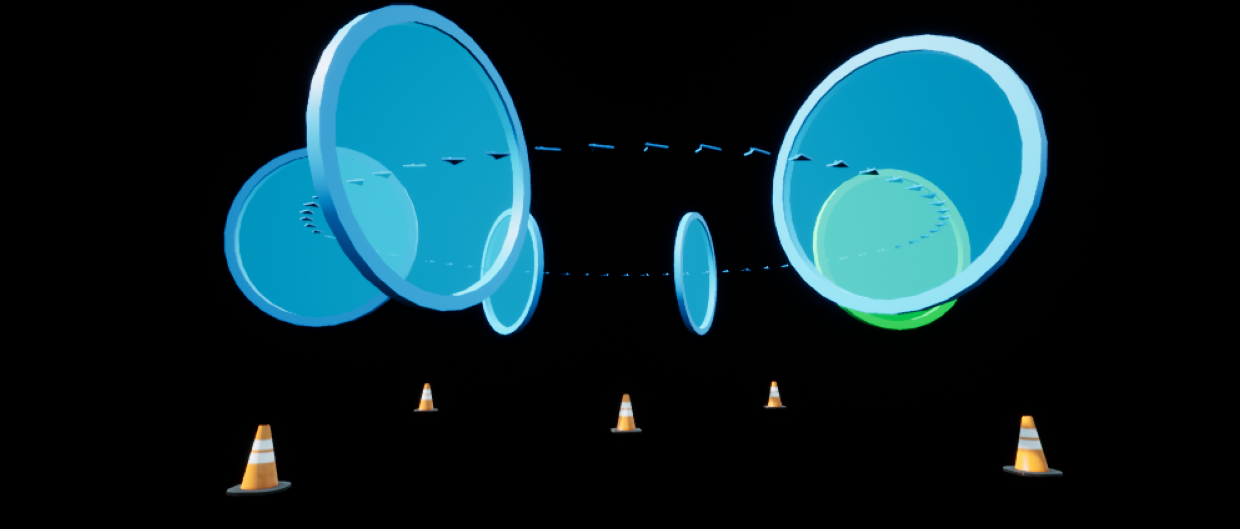
\includegraphics[width=\linewidth]{ar-render.png}
    \caption{Przykład obrazu do wyświetlenia na wyświetlaczu przeziernym}
    \label{fig:ar-render}
\end{figure}

W przypadku aplikacji rzeczywistości rozszerzonej pojawia się nowy problem określenia lokalizacji użytkownika. Urządzenia do wyświetlania aplikacji VR, włącznie z wykorzystywanym w niniejszej pracy Oculus Rift, określają swoją pozycję w przestrzeni wykorzystując pewną liczbę stacjonarnych czujników. Działając na zasadzie stereowizji, możliwe jest prezycyjne i odporne na zaburzenia pozycjonowane gogli w trójwymiarowej przestrzeni. Jeśli w trakcie działania aplikacji użytkownik zmieni swoje fizyczne położenie (na przykład wstanie z fotela), może wykonać tzw. ,,HMD reset'', czyli przyjąć obecne położenie i kierunek patrzenia za referencyjne. Ponieważ wszystkie wyświetlane treści są nierzeczywiste, następujące wtedy przemieszczenie układu współrzędnych wirtualnej sceny względem fizycznego otoczenia nie ma żadnego znaczenia. Ponieważ aplikacje mieszane łączą obraz wygenerowany komputerowo, z widokiem świata zewnętrznego normalnie docierającym do oczu użytkownika, konieczne jest śledzenie położenia względem otaczającego środowiska. W tym celu wykorzystywane są także układy oparte na stereowizji. Umożliwia to na przykład wyświetlanie trójwymiarowych obrazów, które tworzą iluzję jakby stały na stole jak rzeczywiste przedmioty. Wyświetlanie przeszkód i trasy dla BSP generuje dwa główne problemy w śledzeniu pozycji:
\begin{itemize}
    \item brak obiektów referencyjnych --- typowo podczas lotu BSP operator obserwuje go powyżej linii horyzontu
    \item powiązanie układu współrzędnych okularów AR z układem nawigacyjnym BSP
\end{itemize}

Oba powyższe problemy można rozwiązać wprowadzając dodatkowy obiekt dla odniesienia. Może to być zestaw znaczników ArUco \cite{aruco2016}, \cite{aruco2018}, umieszczonych w znanych położeniach w taki sposób aby w trakcie całego lotu przynajmniej jeden z nich pozostawał w polu widzenia kamer dostępnych w urządzeniu AR. Podczas wykonywanych zadań BSP najczęściej znajduje się wyżej niż oczy operatora. Wynika z tego konieczność umieszczenia znaczników na odpowiedniej wysokości, na przykład w sposób zilustrowany na rysunku \ref{fig:aruco}. Na podstawie płaskiego obrazu oraz informacji o głębi z kamery podczerwieni, można na podstawie jednego znacznika rozwiązać zagadnienie estymacji pozy kamery, i w ten sposób związać ją z nieruchomym układem współrzędnych w którym umieszczono znaczniki. Aby poprawnie sprawdzać wystąpienie kolizji oraz liczyć odległość od trasy odniesienia, konieczne jest także związanie lokalnego układu nawigacyjnego BSP z układem rozmieszczenia znaczników. W najprostszy sposób można to osiągnąć poprzez dodanie pola do startu o stałym położeniu względem znaczników. Następnie na tym polu należy umieścić obiekt \emph{SwitchableDrone}, poziomo z osią $ X $ skierowaną w kierunku północnym. Jednak zastosowanie tego rozwiązania wymusza aby każdy lot rozpoczynać od wspomnianego pola startowego. Ten warunek jest konieczny, ale wystarczający, ponieważ w trakcie uruchamiania BSP zapisuje swoją pozycję jako tzw. \emph{HOME}, która staje się punktem zaczepienia lokalnego układu nawigacyjnego \emph{north-east-down}.

\begin{figure}[!h]
    \centering 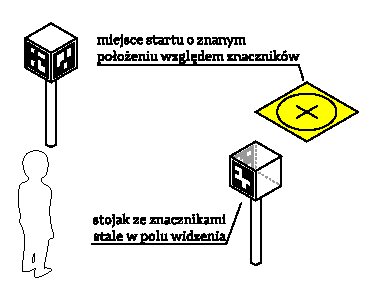
\includegraphics[width=0.8\linewidth]{aruco.pdf}
    \caption{Szkic proponowanego sposobu wzajemnej lokalizacji w trybie AR}
    \label{fig:aruco}
\end{figure}
